\begin{figure}[ht]
  \centerline{
    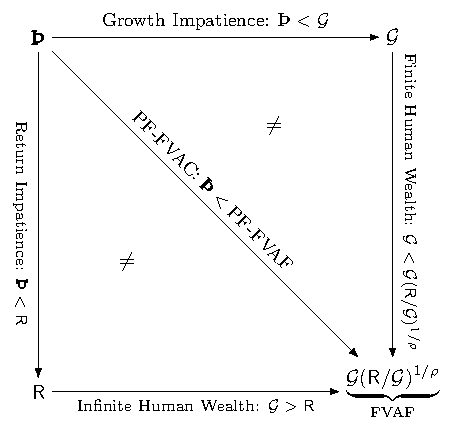
\includegraphics[width=5in]{\FigDir/RelatePFGICFHWCRICPFFVAC}
  }
  \caption{Perfect Foresight Relation of {GIC}, {FHWC}, {RIC}, and {PFFVAC}}
  \iflabelexists{fig:RelatePFGICFHWCRICPFFVAC}{}{\label{fig:RelatePFGICFHWCRICPFFVAC}} % Don't define it if already defined
  \footnotesize{An arrowhead points to the larger of the two quantities being compared; so, the diagonal arrow indicates that absolute patience is smaller than the limit defined by the finite value of autarky factor, $\APFac < \PermGroFac (\Rfree/\PermGroFac)^{1/\CRRA}$ (this is one way of writing the {\PFFVAC}, equation \eqref{eq:PFFVAC}}). (The $\neq$ symbols indicate that the diagram is not commutative; that is, the different ways of reaching the conclusion that the {\PFFVAC} holds are not equivalent to each other).
\end{figure}
